\chapter{Renormalization Group for Ising Model}
\label{renorm-group-ising}



RG theory is intimately linked to
thermodynamics,
and thermodynamics is a world in itself.
Here is but a whiff of thermodynamics.
The \textbf{partition function} $Z$ is defined by

\beq
Z = {\rm tr}(e^{-\beta H})
=\sum_j e^{-\beta E_j}
\;,
\eeq
where $H>0$ is the Hamiltonian matrix
of the system, and $\{E_j\}_j$ are the
eigenvalues of $H$.
The \textbf{free energy}
$F$ is defined in terms
of $Z$ by

\beq
-\beta F = \ln Z
\;,
\label{eq-bridge}
\eeq
 where
$\beta = \frac{1}{k_B T}$,
$k_B$ is Boltzmann's constant, and
$T$ is the temperature of the system.
All the thermodynamic observables
can be expressed in terms of
$F$ and it's derivatives with
respect to $\beta$.
McComb calls Eq.(\ref{eq-bridge})
the \qt{bridge equation},
because it bridges the microscopic physics
with the macroscopic one. 
One could write volumes about $F$
alone. However, since
this is just a brief article,
let's just point out the interesting fact that
at low temperatures (i.e., high $\beta$),
$F \approx E_1$, where $E_1$ is the
lowest (i.e., ground state)
energy of the system.



Let

$Bool=\bool$

$S_i\in \{-1, 1\}= 2Bool-1=\ZZ_\pm$

$S^{:N} =(S_1, S_2, \ldots, S_N)$



Assume $J>0$. The partition function
for a 1-dim Ising model is

\beq
Z = \sum_{S^{:N}\in\ZZ_\pm^N}
e^{-\beta\cale}
\text{ with }
\cale = -J(S_1 S_2 + S_2 S_3 +
S_3 S_4 + \ldots S_{N-1}S_N)
\eeq
Note
that the energy $\cale$ is minimum
iff all spins point
in the same direction.

Let $K=\beta J$.
Then we can rewrite the partition function as
\beq
Z=
\sum_{S^{:N}\in\ZZ_\pm^N}
e^{K(S_1 S_2 +S_2 S_3)}
e^{K(S_3 S_4 +S_4 S_5)}\ldots
\eeq

Let $N'= N/2$. If we sum
the right hand side
of the last equation 
over spins with even indices,
we get

\beq 
Z=
\sum_{S^{:N'}\in\ZZ_\pm^{N'}}
2 \cosh[K(S_1 + S_3)]
2 \cosh[K(S_3 + S_5)]
\ldots
\label{eq-sum-cosh-prod}
\eeq

Next we make the following anzatz
and prove the anzatz is valid
by solving for $f(K)$ and $K'(K)$

\beq
2 \cosh[K(S_1 + S_3)] = f(K) e^{K'(K) S_1 S_3}
\label{eq-1-dim-ising-anzatz}
\eeq


\begin{claim}

\beq
f(K)= 2 \sqrt{\cosh(2K)}
\eeq
 \beq
K'=\frac{1}{2}\ln[\cosh(2K)]
\quad\text{(plotted in Fig.\ref{fig-kprime-versus-k})}
\label{eq-1dim-ising-kprime-k}
\eeq
Hence for a 1-dim Ising model,

\beq
\left\{
\begin{array}{l}
\text{$K'(K=0)= 0$}
\\
\text{As $K'\rarrow \infty$, $K'\rarrow K -\frac{1}{2}\ln(2)\rarrow K$}
\end{array}
\right.
\eeq 

\end{claim}
\proof

From the anzatz Eq.(\ref{eq-1-dim-ising-anzatz}),
we get
\beq
f(K)=
e^{-K' S_1 S_3}\left
[e^{K(S_1+S_3)}
+
e^{-K(S_1+S_3)}
\right]
\eeq

\begin{subequations}\label{eq-1-dim-ising-2eqs}
When $S_1$ and $S_3$ point in the
same direction,

\beq
f(K)=e^{-K'}\left[e^{2K}+ e^{-2K}\right]
\eeq
When $S_1$ and $S_3$ point in opposite
directions,

\beq \label{eq-1-dim-ising-easy}
f(K)=e^{K'}2
\eeq
\end{subequations}

Dividing the 2 equations Eqs.(\ref{eq-1-dim-ising-2eqs}) yields

\beq
e^{2K'}=\cosh(2K)
\eeq
Now that we know $K'(K)$,
we can find $f(K)$
from Eq.(\ref{eq-1-dim-ising-easy}).
\qed

Combining Eq.(\ref{eq-sum-cosh-prod}) and
the anzatz Eq.(\ref{eq-1-dim-ising-anzatz}),
we get
\beq
\underbrace{Z}_{Z(N, K)}=f^{N'}(K)\underbrace{\sum_{S^{:N'}\in \ZZ_\pm} 
e^{K'S_1 S_3}e^{K'S_3 S_5}\ldots}_{
Z(N', K')
}
\label{eq-z-prior-use-extensive}
\eeq

For large $N$,
\beq
\ln Z \approx \sum_{S^{:N}\in\ZZ_\pm^N}
 \ln e^{-N\beta \cale_1}=N\zeta(K)
\eeq
so $\ln Z$ behaves as an extensive variable.
By virtue of this extensive property,
Eq.(\ref{eq-z-prior-use-extensive}) 
becomes

\beq
N\zeta(K)= N'\ln f(K) + N'\zeta(K')
\eeq
so

\beq
\zeta(K') = 2\zeta(K)- \ln f(K)
\eeq
where 

\beq
\ln f(K)=\frac{1}{2}\ln \cosh(2K) + \ln 2
\eeq


Instead of Eq.(\ref{eq-1dim-ising-kprime-k}), 
for a 2-dim Ising model, it
has been shown that

\beq
K'\approx \frac{3}{8}\ln[\cosh(4K)]
\quad\text{(plotted in Fig.\ref{fig-kprime-versus-k})}
\eeq

Hence, for a 2-dim Ising model

\beq
\left\{
\begin{array}{l}
\text{$K'(K=0)= 0$}
\\
\text{As $K'\rarrow \infty$, $K'\rarrow \frac{3}{2}K -\frac{3}{2}\ln(2)\rarrow \frac{3}{2}K$ }
\end{array}
\right.
\eeq

\begin{figure}[h!]
\centering
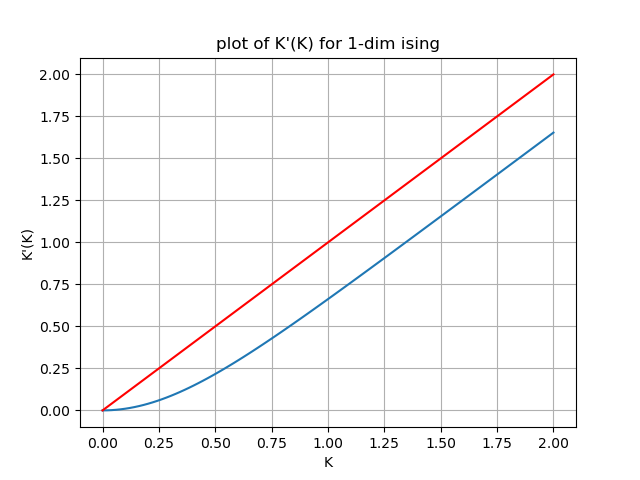
\includegraphics[width=3.5in]
{renorm-group-intro/kprime-versus-k-1dim-ising.png}
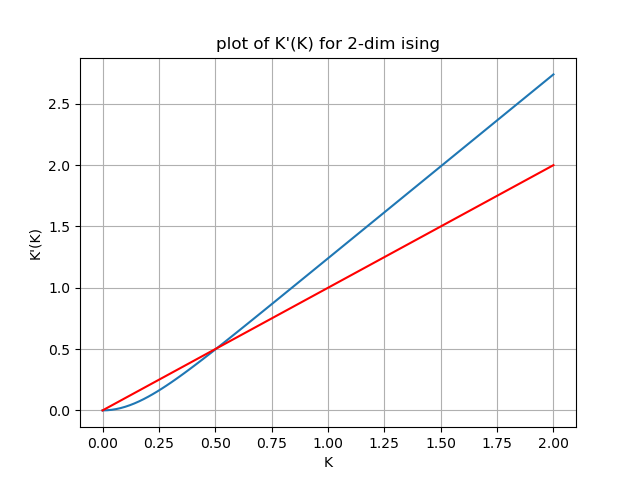
\includegraphics[width=3.5in]
{renorm-group-intro/kprime-versus-k-2dim-ising.png}
\caption{Plots of $K'(K)$ (in blue) 
for 1-dim and 2-dim Ising model.
Line $K'=K$ in red.}
\label{fig-kprime-versus-k}
\end{figure}

\begin{figure}[h!]
\centering
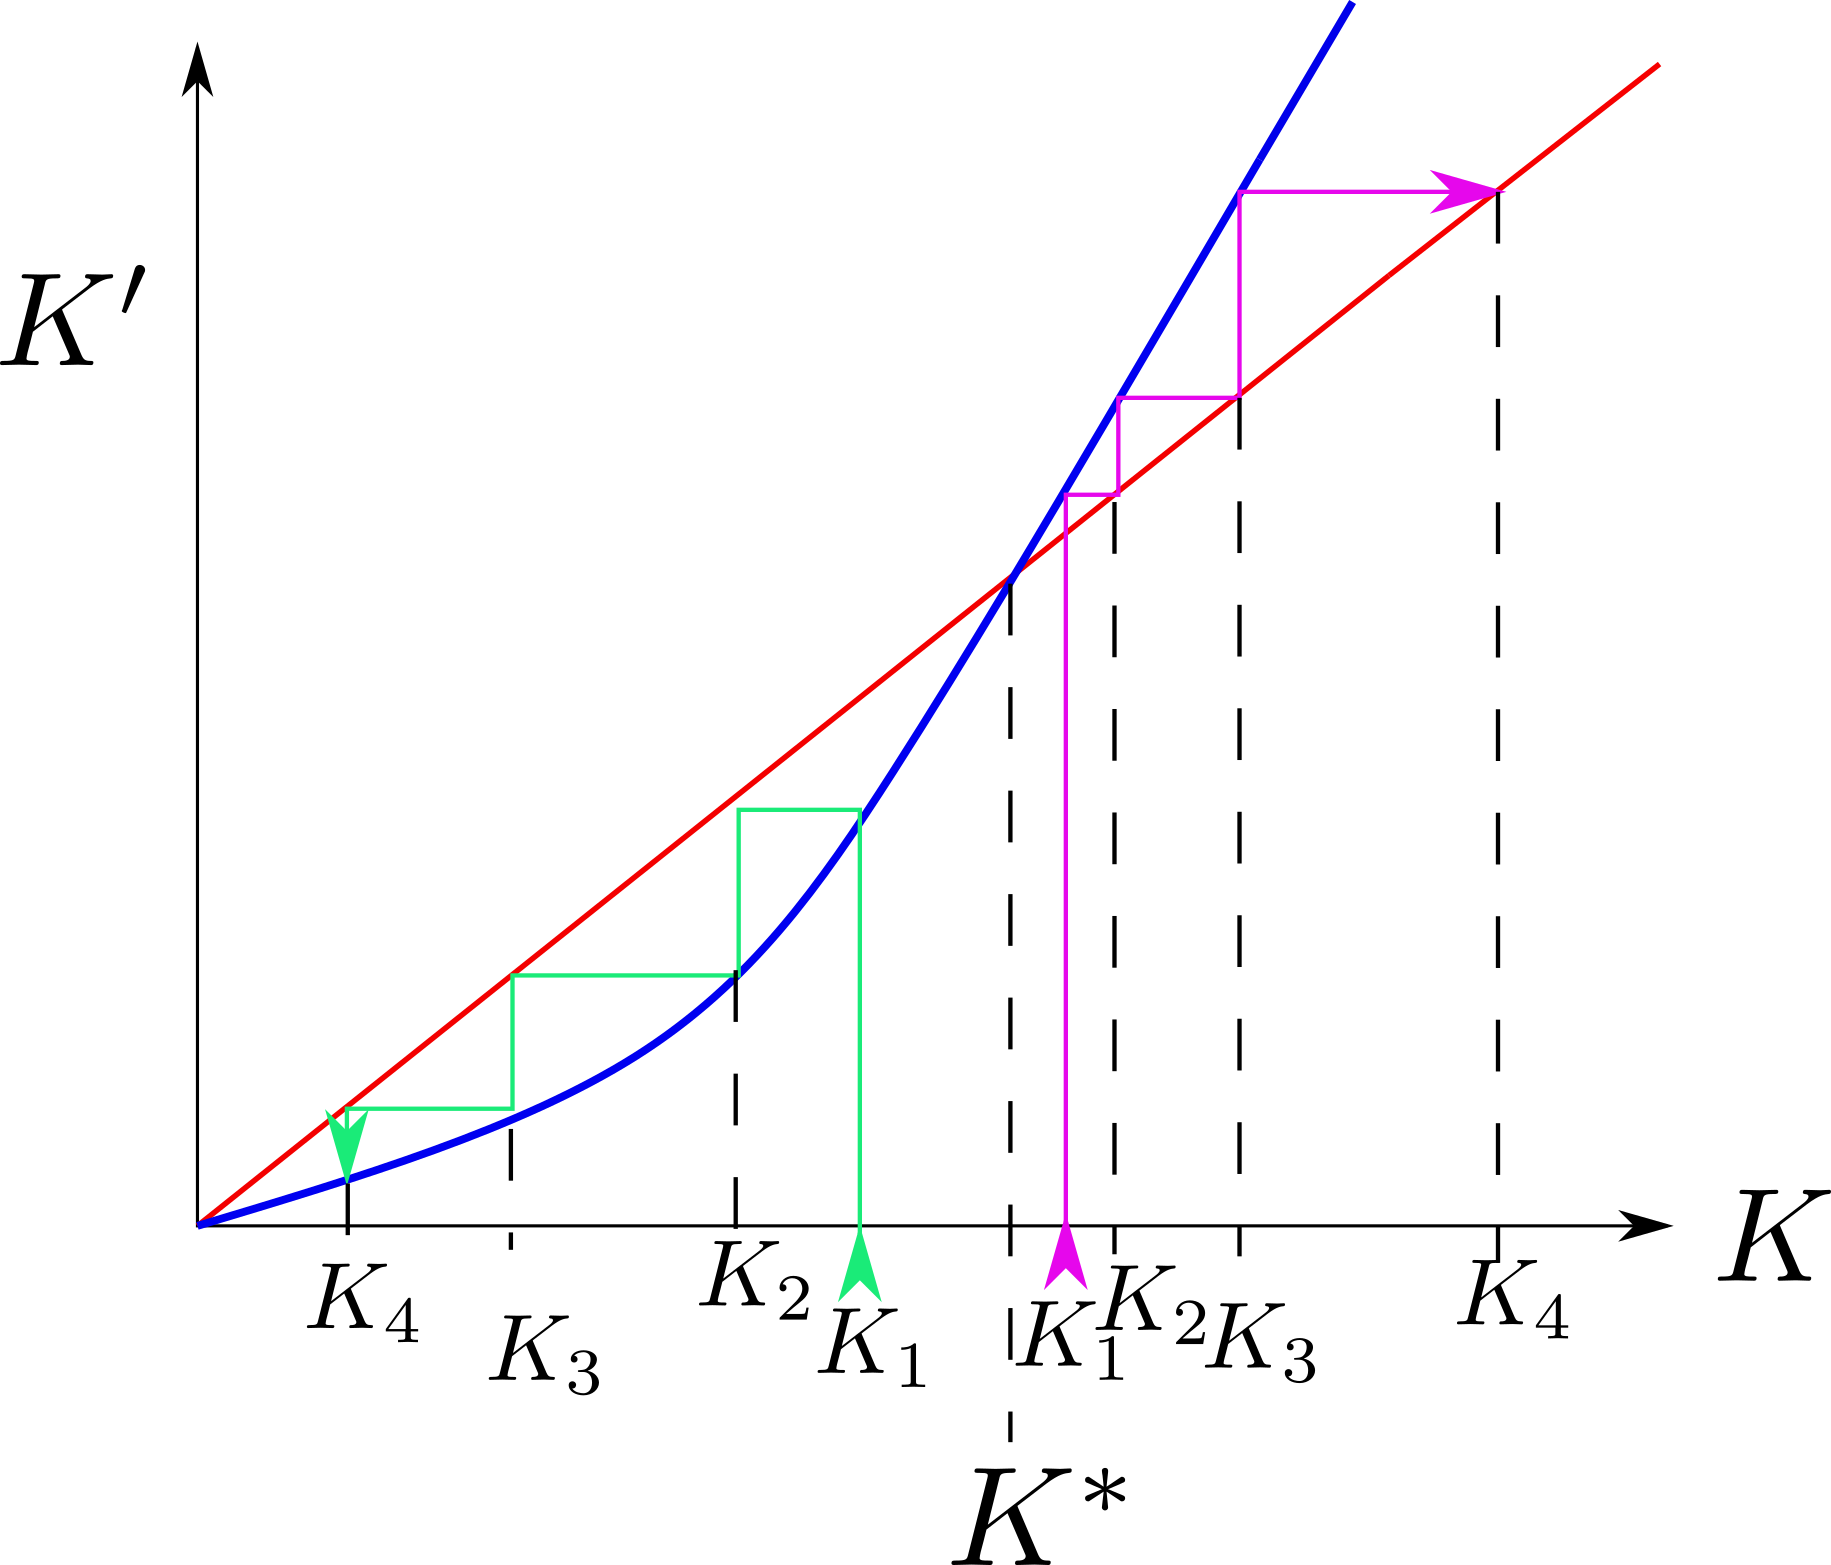
\includegraphics[width=3.5in]
{renorm-group-intro/repeller-rg.png}
\caption{Schematic of $K'(K)$ (in blue)
for 2-dim Ising model. Red line is line
$K'=K$. The point with $K=K^*$ where the red and blue lines intersect
is the critical point.
By applying the RG transformation $K(K')$
recursively
3 times, starting with $K_1$, we get $K_1, K_2, K_3, K_4$.}
\label{fig-repeller-rg}
\end{figure}

As can be seen from Figs.\ref{fig-kprime-versus-k} and
\ref{fig-repeller-rg},
the 1-dim Ising model has no fixed (critical)
point, but the 2-dim Ising model does.

